\documentclass{article}
\usepackage[margin=1in]{geometry}
\usepackage{problemset}
\showsolntrue

% Custom commands
\newcommand{\R}{\mathbb{R}}
\newcommand{\X}{\mathcal{X}}
\newcommand{\Y}{\mathcal{Y}}
\newcommand{\E}{\mathbb{E}}
\newcommand{\V}{\text{Var}}
\renewcommand{\P}{\mathbb{P}}
\newcommand{\x}{\mathbf{x}}
\newcommand{\w}{\mathbf{w}}
\newcommand{\h}{\mathbf{h}}
\newcommand{\W}{\texttt{W}}
\renewcommand{\b}{\mathbf{b}}
\newcommand{\y}{\mathbf{y}}
\newcommand{\z}{\mathbf{z}}

\begin{document}

\pstitle{%
    COGS 181%
}{
    Homework 3%
}[due Tuesday, February 10, 2026 at 11:59PM]

\textbf{Instructions:} Answer the questions below, attach your code, and insert figures to create a PDF file; submit your file via Gradescope. You may look up the information on the Internet, but you must write the final homework solutions by yourself.

\textbf{Late Policy:} 5\% of the total points will be deducted on the first day past due. Every 10\% of the total points will be deducted for every extra day past due.


\begin{probset}
% --- Problem 1 ---
\begin{prob}[\textbf{(14 points) Conceptual Questions}]
    \begin{subprobset}
        \begin{subprob}
            Is the following statement true or false?

            Suppose the perceptron algorithm has computed a classifier parameterized by $\w$. Now, consider a new weight vector $\w' = c\w$ where $c$ is a nonzero scalar. Assume that the bias is zero. Using $\w'$ instead for classification might result in a different decision function.

            \begin{soln}
                True, if $c < 0$, the decision will be different since the sign of $\w' \cdot \x$ will be different.
            \end{soln}
        \end{subprob}

        \begin{subprob}
            \textbf{True or False.} For a two-layer neural network, if we increase the total number of neurons by adding one more hidden layer, then the test error of the new neural network can \textbf{always} be decreased.

            \begin{soln}
                False. There are a number of reasons why the test error may not decrease.
            \end{soln}
        \end{subprob}

        \begin{subprob}
            \textbf{True or False.} Suppose we design two alternative multi-layer neural network architectures to solve a classification problem. Let these two neural networks have the \textbf{same number of neurons}. If both are successfully trained on the same training set, then the deeper multi-layer neural network will always result in a smaller training error than the shallower one.

            \begin{soln}
                False. This is not always the case for a number of reasons.
            \end{soln}
        \end{subprob}

        \begin{subprob}
            \textbf{True or False.} The choice of the type of activation function in a multi-layer neural network affects how easily it can be trained \textbf{but not} the final training error of the classifier.

            \begin{soln}
                False. The choice of the type of activation function affects both the final training error and the difficulty in training.
            \end{soln}
        \end{subprob}

        \begin{subprob}
            \textbf{True or False.} The choice of the type of activation function in a multi-layer neural network decides the final training error of the classifier \textbf{but not} the difficulty in training.

            \begin{soln}
                False. The choice of the type of activation function affects both the final training error and the difficulty in training.
            \end{soln}
        \end{subprob}

        \newpage

        \begin{subprob}
            Choose the \textbf{most} significant difference between the \textbf{backpropagation} process in multi-layer neural networks and the \textbf{training process} in the logistic regression algorithm:

            \begin{enumerate}[label=\Alph*.]
                \item deal with unsupervised learning vs. supervised learning
                \item used with softmax function vs. sigmoid function
                \item train networks with hidden layers vs. without hidden layers
                \item used with gradient descent vs. closed-form solution
            \end{enumerate}

            \begin{soln}
                C is the most significant difference. Logistic regression doesn't have hidden layers, while backpropagation is used to train networks with hidden layers.
            \end{soln}
        \end{subprob}

        \begin{subprob}
            Kevin and John are having an argument about the backpropagation algorithm. Kevin claims that in backpropagation, first all the gradients with respect to weights in \textbf{all layers} are calculated and then all weights are updated simultaneously. John argues that the weights for \textbf{each layer} should be updated as soon as the gradients for the layer are computed, and then compute the gradients for the previous layer using updated weights. Which one of them is more favorable?

            \begin{soln}
                Kevin is more favorable. You should compute the gradients for all layers at once, and then update the weights.
            \end{soln}
        \end{subprob}
    \end{subprobset}
\end{prob}

% --- Problem 2 ---
\begin{prob}[\textbf{(15 points) Back-Propagation in Neural Networks}]
    In this problem, we will derive necessary gradients for training the network of Figure 1 by backpropagation. \textbf{If you have already finished this question using Option 1 (the original form), you don't need extra work. If you have just started working on this problem, please take option 2, which is in a simpler form.}

    \textbf{Option 1 (original form):} You can assume all variables are in matrix/vector form $\x \in
    \R^{m \times 1}$, $\w_1, \w_2 \in \R^{m \times h}$, $\h_1, \h_2 \in \R^{h \times 1}$, $\h \in \R^{2h \times 1}$, $\w_3, \w_4 \in \R^{2h \times n}$.

    \textbf{Option 2 (simpler form [new]):} You can assume all variables are in vector/scalar form $\x \in \R^m$, $\w_1 \in \R^m$, $\w_2 \in \R^m$, $\h \in \R^2$, $\w_3 \in \R^2$, $\w_4 \in \R^2$, $h_1$ and $h_2$ are scalars.

    \[ \sigma(\w, \x) = \frac{1}{1 + e^{-\w^\top \x}} \]

    \textbf{Hint:}
    \begin{enumerate}
        \item Use the chain rule to answer the questions in terms of the variables in the graph.
        \item Use the gradient of the sigmoid function.
    \end{enumerate}

    \begin{figure}[H]
        \centering
        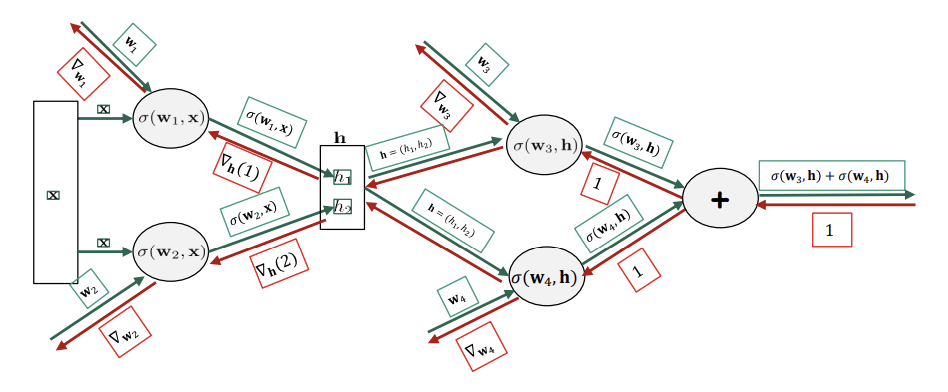
\includegraphics[width=0.8\textwidth]{Images/fig1.png}
        \caption{Question 4}
    \end{figure}

    \begin{subprobset}
        \begin{subprob}
            \textbf{(3 points)} Compute $\nabla_{\w_4}$.

            \begin{soln}
                $\nabla_{\w_4} = \frac{\partial}{\partial \w_4} \sigma(\w_4, \h) = \sigma(\w_4, \h) (1 - \sigma(\w_4, \h)) \h$
            \end{soln}
        \end{subprob}

        \begin{subprob}
            \textbf{(3 points)} Compute $\nabla_{\w_3}$.

            \begin{soln}
                $\nabla_{\w_3} = \frac{\partial}{\partial \w_3} \sigma(\w_3, \h) = \sigma(\w_3, \h) (1 - \sigma(\w_3, \h)) \h$
            \end{soln}
        \end{subprob}

        \begin{subprob}
            \textbf{(3 points)} Compute $\nabla_{\h}$.

            \begin{soln}
                $\nabla_{\h} = \frac{\partial}{\partial \h} (\sigma(\w_4, \h) + \sigma(\w_3, \h)) = \sigma(\w_4, \h) (1 - \sigma(\w_4, \h)) \w_4 + \sigma(\w_3, \h) (1 - \sigma(\w_3, \h)) \w_3$
            \end{soln}
        \end{subprob}

        \begin{subprob}
            \textbf{(3 points)} Compute $\nabla_{\w_2}$ in terms of $\nabla_{\h} (2)$

            \begin{soln}
                $\nabla_{\w_2} = \frac{\partial}{\partial \w_2} \sigma(\w_2, \x) \cdot \nabla_{\h} (2) = \sigma(\w_2, \x) (1 - \sigma(\w_2, \x)) \x \cdot \nabla_{\h} (2)$
            \end{soln}
        \end{subprob}

        \begin{subprob}
            \textbf{(3 points)} Compute $\nabla_{\w_1}$ in terms of $\nabla_{\h} (1)$

            \begin{soln}
                $\nabla_{\w_1} = \frac{\partial}{\partial \w_1} \sigma(\w_1, \x) \cdot \nabla_{\h} (1) = \sigma(\w_1, \x) (1 - \sigma(\w_1, \x)) \x \cdot \nabla_{\h} (1)$
            \end{soln}
        \end{subprob}
    \end{subprobset}
\end{prob}

\newpage

% --- Problem 3 ---
\begin{prob}[\textbf{(7 points) Softmax Classification}]
    In this section, we consider the multi-class classification problem: We need to predict a K-way label $\hat{y} \in \{0, 1, ..., K - 1\}$ for each input $\x = (x_0, ..., x_{D-1})^\top$. Note that we represent the $K$ classes by $\{0, 1, ..., K - 1\}$ instead of $\{1, ..., K\}$ in lecture slides because it is easier to implement in Python. Then, we can express the conditional probability (or confidence) of class $j$ parameterized by $\W = (\w_0, ..., \w_{K-1})^\top \in \R^{K \times D}$ and $\b = (b_0, ..., b_{K-1})^\top \in \R^{K}$ as

    \[ p_j = p(y = j|\x) = \frac{e^{f_j}}{\sum_{k=0}^{K-1} e^{f_k}} \]

    where $f_j = \w_j \x + b_j$.

    We choose the class with the highest probability among all $K$ classes as the prediction $\hat{y}$:

    \[ \hat{y} = \text{argmax}_j p_j = \text{argmax}_j p(y = j|\x) \]

    In the training process, given a data point $\{(\x, y)\}$ in the training set, we firstly rewrite the label $y \in \{0, 1, ..., K - 1\}$ in the one-hot encoding form $\y \in \R^K$:

    \[ \y = (y_0, ..., y_{K-1})^\top, \text{where } y_j = \begin{cases} 1 & \text{if } j = y \\ 0 & j \neq y \end{cases} \]

    Then, we wish to optimize the following cross-entropy loss on the data point $\{(\x, y)\}$:

    \[ L(\x, y; \W, \b) = -\ln p_y = -\sum_{l=0}^{K-1} y_l \ln p_l \]

    Given the training dataset $\{(\x^{(i)}, y^{(i)})\}$, we sum the cross-entropy losses over all data points in the dataset:
    \[ L(\W, \b) = \sum_{i=1}^n L(\x^{(i)}, y^{(i)}; \W, \b) \]

    In this problem, we will minimize $L(\W, \b)$ using gradient descent and obtain the optimal $\W^*$ and $\b^*$.

    Please derive the following:

    \newpage

    \begin{subprobset}
        \begin{subprob}
            \textbf{(5 points)} For one data point $\{(\x, y)\}$, show that the gradient of $L(\x, y; \W, \b)$ with respect to the $f_j$ is given by:

            \[ \frac{\partial L(\x, y; \W, \b)}{\partial f_j} = p_j - y_j \]

            \begin{soln}
                Let $L = -\sum_{l=0}^{K-1} y_l \ln p_l$, $Z = \sum_{k=0}^{K-1} e^{f_k}$, and $
                \delta_{lj} = \textbf{1}(l = j)$. Then,
                \begin{align*}
                    \frac{\partial L}{\partial f_j}
                    &= -\sum_{l=0}^{K-1} y_l \frac{\partial \ln p_l}{\partial f_j}
                    = -\sum_{l=0}^{K-1} y_l \left( \delta_{lj} - \frac{e^{f_j}}{Z} \right)
                    = -\sum_{l=0}^{K-1} y_l (\delta_{lj} - p_j) \\
                    &= -y_j + p_j \sum_{l=0}^{K-1} y_l
                    = -y_j + p_j
                    = p_j - y_j
                \end{align*}
            \end{soln}
        \end{subprob}

        \begin{subprob}
            \textbf{(2 points)} Assume $\w_j = (w_{j0}, ..., w_{j(D-1)})^\top$, show that the gradient of $L(\x, y; \W, \b)$ with respect to the $w_{jd}$ and $b_j$ is given by:
            \[ \frac{\partial L(\x, y; \W, \b)}{\partial w_{jd}} = (p_j - y_j) x_d \qquad \frac{\partial L(\x, y; \W, \b)}{\partial b_j} = p_j - y_j \]

            \begin{soln}
                \begin{align*}
                    \frac{\partial L}{\partial w_{jd}}
                    &= \frac{\partial L}{\partial f_j} \cdot \frac{\partial f_j}{\partial w_{jd}}
                    = (p_j - y_j) \cdot x_d
                \end{align*}
                \begin{align*}
                    \frac{\partial L}{\partial b_j}
                    = \frac{\partial L}{\partial f_j} \cdot \frac{\partial f_j}{\partial b_j}
                    = (p_j - y_j) \cdot 1
                    = p_j - y_j
                \end{align*}
            \end{soln}
        \end{subprob}
    \end{subprobset}
\end{prob}

\newpage

% --- Problem 4 ---
\begin{prob}[\textbf{(12 points) Feed-Forward Neural Network}]
    In this question, on top of the single-layer network, we add another layer between the input and output with the sigmoid activation function, and this hidden layer contains 3 \textbf{hidden units}. Assume an input feature $\x \in \R^{2 \times 1}$. Thus, the probability of output $y$ is represented as:

    \[ p(y|\x) = \sigma \left( y \times (\w_2^\top \sigma(\W_1^\top \x + \b_1) + b_2) \right) \]

    where $\W_1 \in \R^{2 \times 3}$ and $\w_2 \in \R^{3 \times 1}$ are the weights, $\b_1 \in \R^{3 \times 1}$ and $b_2 \in \R^{1 \times 1}$ are the biases. The activation function is the logistic sigmoid function, which is defined as follows:

    \[ \sigma(z) = \frac{1}{1 + e^{-z}} \]

    The logistic sigmoid function is applied on each entry in the vector or matrix. For example, we define $\h = \sigma(\W_1^\top \x + \b_1)$ as the output of the first layer. The output of $\W_1^\top \x + \b_1$ is a 3-dimension vector, and the sigmoid function $\sigma(\cdot)$ is applied at each entry of the 3-dimension vector, so $\h$ is still a 3-dimension vector (i.e. $\h \in \R^{3 \times 1}$).

    In order to train a binary classifier with this network, we define a cross-entropy loss function to measure the distance between the target and the prediction from this network, and the loss function $L$ for one point $(\x, y)$ is defined as:

    \[ L(\W_1, \w_2, \b_1, b_2) = -\ln p(y|\x) \]

    In the training process, we aim to minimize the loss function $L_{\text{train}}$ over the training set \newline $S_{\text{train}} = \{(\x^{(0)}, y^{(0)}), ..., (\x^{(n-1)}, y^{(n-1)})\}$:

    \[ L_{\text{train}}(\W_1, \w_2, \b_1, \b_2) = -\sum_{i=0}^{n-1} \ln p(y^{(i)}|\x^{(i)}) \]

    Since there is no closed-form solution for the weights and the bias in the network, we consider a gradient descent algorithm to train the network. 
    
    Assume $p = p(y|\x)$, please prove the following:

    \newpage

    \begin{subprobset}
    \begin{subprob}
        $\displaystyle\frac{\partial L}{\partial \w_2} = (p - 1) y \times \h$

        \begin{soln}
            Let $z = y \times (\w_2^\top \h + b_2)$ so $p = \sigma(z)$. Then $\frac{\partial z}{\partial \w_2} = y\h$ and
            
            \begin{align*}
                \frac{\partial L}{\partial z} = -
                \frac{\partial}{\partial z} \ln p = -\frac{1}{p} \cdot p (1 - p) = p - 1
            \end{align*}
            \begin{align*}
                \frac{\partial L}{\partial \w_2}
                &= \frac{\partial L}{\partial z} \cdot \frac{\partial z}{\partial \w_2}
                = (p - 1) \cdot y \cdot \h
            \end{align*}
        \end{soln}
    \end{subprob}

    \begin{subprob}
        $\displaystyle\frac{\partial L}{\partial b_2} = (p - 1) y$

        \begin{soln}
            Using the same $z = y \times (\w_2^\top \h + b_2)$, we have $\frac{\partial z}{\partial b_2} = y$. Hence,

            \begin{align*}
                \frac{\partial L}{\partial b_2}
                &= \frac{\partial L}{\partial z} \cdot \frac{\partial z}{\partial b_2}
                = (p - 1) \cdot y
            \end{align*}
        \end{soln}
    \end{subprob}

    \begin{subprob}
        $\displaystyle\frac{\partial L}{\partial \h} = (p - 1) y \times \w_2$

        \begin{soln}
            Using the same $z = y \times (\w_2^\top \h + b_2)$, we have $\frac{\partial z}{\partial \h} = y\w_2$. Hence,

            \begin{align*}
                \frac{\partial L}{\partial \h}
                &= \frac{\partial L}{\partial z} \cdot \frac{\partial z}{\partial \h}
                = (p - 1) \cdot y \cdot \w_2
            \end{align*}
        \end{soln}
    \end{subprob}
    \end{subprobset}
\end{prob}

\newpage

% --- Problem 5 ---
\begin{prob}[\textbf{(12 points) 2-D Convolution}]
    Suppose we have a small network for image recognition. The input image $\x \in \R^{4 \times 4}$. The network has three layers named Conv, MaxPool, and ReLU:

    \[ \text{Image} \x \to \text{Conv} \xrightarrow{\z_1} \text{MaxPool} \xrightarrow{\z_2} \text{ReLU} \rightarrow \z_3 \]
    
    where $\z_1, \z_2$ are intermediate output and $\z_3$ is the final output. The details of the layers are given below:
    \begin{itemize}[label={}]
        \item \textbf{Conv:} A single-channel convolution layer with 3$\times$3 kernel, stride size 1 and no padding.
        \item \textbf{MaxPool:} A max pooling layer with 2$\times$2 kernel and stride size 2.
        \item \textbf{ReLU:} A ReLU activation layer which has $\max(0, z)$ as the output of input $z$.
    \end{itemize}

    \begin{subprobset}
        \begin{subprob}
            \textbf{(6 points) Output Shape Computation}

            Please calculate the shape of the outputs and fill in the blanks below:

            \begin{enumerate}
                \item Shape of input $\x$: 4 $\times$ 4.
                \item Shape of intermediate output $\z_1$: \_\_\_\_\_\_ $\times$ \_\_\_\_\_\_ .
                \item Shape of intermediate output $\z_2$: \_\_\_\_\_\_ $\times$ \_\_\_\_\_\_ .
                \item Shape of final output $\z_3$: \_\_\_\_\_\_ $\times$ \_\_\_\_\_\_ .
            \end{enumerate}

            \begin{soln}
                \begin{enumerate}
                    \item Shape of input $\x$: 4 $\times$ 4.
                    \item Shape of intermediate output $\z_1$: 2 $\times$ 2.
                    \item Shape of intermediate output $\z_2$: 1 $\times$ 1.
                    \item Shape of final output $\z_3$: 1 $\times$ 1.
                \end{enumerate}
            \end{soln}
        \end{subprob}

        \begin{subprob}
            \textbf{(6 points) Output Value Computation}

            \begin{center}
                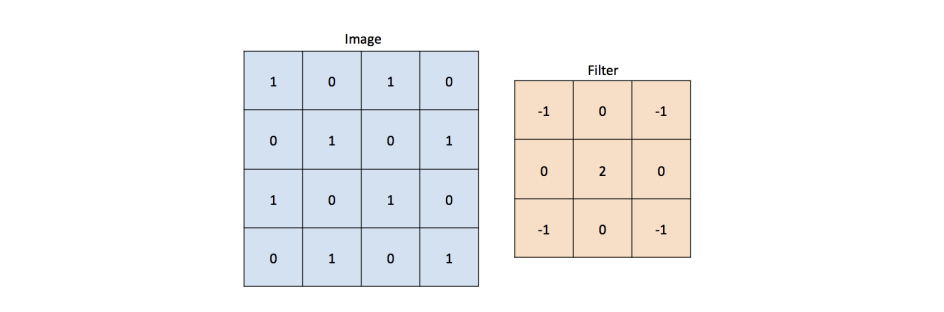
\includegraphics[width=0.7\textwidth]{Images/fig2.png}
            \end{center}

            Assume the values of input image $\x$ and the filter of the Conv layer are given in the figure above. Please compute the values of outputs $\z_1$, $\z_2$ and $\z_3$ by hand.
            
            \textbf{Hint:} The values of $\z_1$, $\z_2$ and $\z_3$ should match the shapes in the previous sub-problem.

            \begin{soln}
                \begin{align*}
                    \z_1 &= \begin{bmatrix}
                        -2 & 0 \\
                        0 & -2
                    \end{bmatrix} \\
                    \z_2 &= \max(z_1) = \max(0, -2) = 0 \\
                    \z_3 &= \max(0, 0) = 0
                \end{align*}
            \end{soln}
        \end{subprob}
    \end{subprobset}
\end{prob}

\newpage

\fontsize{12pt}{\baselineskip}\selectfont\textbf{Programming Part}

Question 6 and 7 are coding questions. Please refer to the Jupyter notebook \texttt{hw3.ipynb}.

% --- Problem 6 ---
\begin{prob}[\textbf{(20 points) Softmax Classification}]\end{prob}

% --- Problem 7 ---
\begin{prob}[\textbf{(20 points) Feed-Forward Neural Network}]\end{prob}
\end{probset}
\end{document}